\documentclass[twocolumn]{IEEEtran}
\usepackage{graphicx}
\usepackage[utf8x]{inputenc}
\usepackage{times}
\usepackage{amssymb,amsfonts}
\usepackage{pict2e}
\usepackage{float}
\usepackage[all]{xy}
\usepackage{graphics,graphicx,color,colortbl}
\usepackage{subfigure}
\usepackage{wrapfig}
\usepackage{multicol}
\usepackage{cite}
\usepackage{url}
\usepackage[tbtags]{amsmath}
\usepackage{amsmath,amssymb,amsfonts,amsbsy}
\usepackage{bm}
\usepackage{listings}
\usepackage{algorithm}
\usepackage{algorithmic}
\usepackage[centerlast, small]{caption}
\usepackage[colorlinks=true, citecolor=blue, linkcolor=blue, urlcolor=blue, breaklinks=true]{hyperref}
\hyphenation{ele-men-tos he-rra-mi-en-ta cons-tru-yen trans-fe-ren-ci-a}

%\texttrademark : pone el símbolo TM
%\textregistered : pone el símbolo consistente en una R rodeada de un círculo
%\textcopyright : pone el símbolo consistente en una C rodeada de un círculo


\begin{document}
\title{Modelado e Identificación}
\author{Israel Ricardo Bernal Sánchez Código: $261613$\\
	Felipe Castañeda Prieto Código $285728$\\
	David Ricardo Martínez Hernández Código: $261931$\\
	Oscar Andrés Urbano Vallejo Código: $261683$}
\maketitle
\markboth{Universidad Nacional de Colombia}{}
\floatname{algorithm}{Algoritmo}
\begin{abstract}
 En esta práctica se obtuvo el modelo mediante  función de transferencia de diferentes sistemas, esto se hizo a través de la determinación de parámetros visuales, y mediante el uso de herramientas de cómputo como Ident de Matlab. Además se compararon las diferentes funciones de transferencia obtenidas por los diferentes métodos, con el fin de obtener el modelo que mejor describa el comportamiento del sistema.
\end{abstract}

\begin{keywords}
 Función de transferencia, Ident, Modelo, Respuesta transitoria, Simulink.
\end{keywords}

\section{Introducción}
\noindent
La presente práctica se centra en encontrar la función de transferencia que mejor describa un sistema, esto puede hacerse a través del uso de herramientas de cómputo y métodos gráficos. Sin embargo cómo se verá más adelante, las herramientas computacionales (como Ident de Matlab) ofrecen el mejor método para la obtención de dichos modelos, permitiendo elegir el orden de la función de transferencia que se piensa obtener, las condiciones iniciales, o incluso retrasos en el tiempo de respuesta.

\section{Procedimiento}
\noindent
Análisis y modelado usando Matlab$^{\textregistered}$, Análisis de respuesta transitoria y modelado experimental del motor LEGO, y Modelado de motores DC.

\subsection{Análisis y Modelado usando Matlab$^{\textregistered}$}
\noindent
Los parámetros hallados son los siguientes:
\begin{itemize}
 \item $k= 2.015s$
 \item $M_p=0.3782$
 \item $\zeta=0.2957$
 \item $\omega_n=1.0361$
 \item $t_s=8.41s$
\end{itemize}
\begin{equation}
 G(s)=\frac{Y(s)}{U(s)}=\frac{{k\omega _n ^2 }}{{s_2  + 2\varsigma \omega _n s + \omega _n ^2 }}
\label{ecu10}
\end{equation}
\noindent
Hacienda uso de la ecu. \ref{ecu10} se determinó la función de transferencia del sistema, suponiendo un sistema de segundo orden:
$$\frac{{2.1631}}{{s^2  + 0.6127s + 1.0735}} = \frac{{2.015}}{{0.9315s^2  + 0.5707s + 1}}$$
\noindent
3. Compare la respuesta del modelo que obtuvo en el punto anterior con la respuesta real Fig. \ref{fig13}
\begin{figure}[]
	\centering
		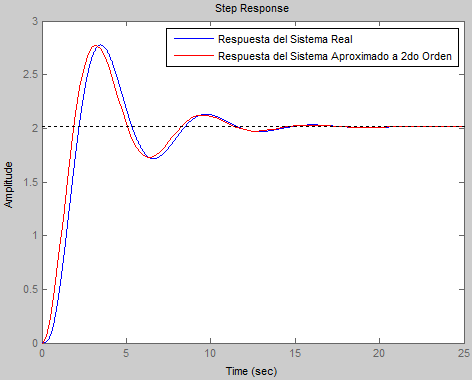
\includegraphics[scale=0.5]{figure13.png}
	\caption{Comparación, respuesta real y modelo}
	\label{fig13}
\end{figure}
\noindent
De la gráfica se observa que el modelo de segundo orden no es el mejor, este se puede mejorar aumentando un polo al modelo, esto se hace en el siguiente punto.\\\\
De la gráfica de la Fig. \ref{fig13} se observa que a pesar de la semejanza de ambas funciones, el sistema real no es de segundo orden (lo que se evidencia en la forma en que empieza la señal real), por ello se hace una segunda aproximación mediante un segundo modelo, esta vez se aumenta un polo más de manera que el modelo resultante es de tercer orden, el polo se ubica en $s= - 4$ esto genera la siguiente función de transferencia:
$$G_b(s)=\frac{2.209}{0.25s^3+1.156s^2+0.8929s+1.096}$$
Se compara ahora el sistema real con el modelo modificado
\begin{figure}[]
	\centering
		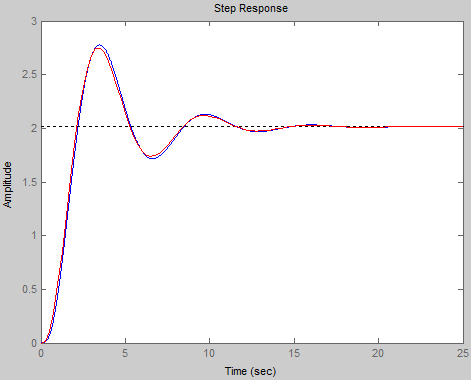
\includegraphics[scale=0.5]{figure14.png}
	\caption{Comparacion, respuesta real y Modelo2}
	\label{fig14}
\end{figure}
\noindent
En la Fig. \ref{fig14} se observa que aumentado el tercer polo el modelo se aproxima mucho más al real.\\\\
Mediante el uso de Ident se obtuvieron dos modelos, el primero con $2$ polos (P$2$U) y el segundo con $3$ polos (P$3$U), esto con el fin de analizar la influencia de un tercer polo esta vez en la aproximación hecha por computador, las funciones de transferencia se muestran a continuación:
\begin{equation}
 G_2(s)\frac{2.013}{0.9281s^2+0.5658s+1}
\end{equation}
\begin{equation}
 G_3(s)\frac{10.18}{s^3+5.234s^2+3.869s+5.053}
\end{equation}
\noindent
En la Fig. \ref{fig15} se observa que ambas repuestas tienen una aproximación a la figura real muy buena, se podría decir que el efecto de un tercer polo en este caso no influencio mucho el modelo debido a que la primera aproximación ($2$ polos) realizada  es casi perfecta.
\begin{figure}[H]
	\centering
		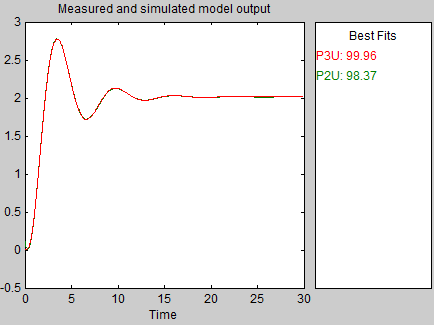
\includegraphics[scale=0.5]{figure15.png}
	\caption{Modelos generados a través de Ident}
	\label{fig15}
\end{figure}
\begin{figure}[H]
	\centering
		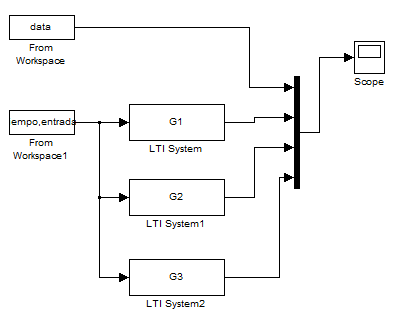
\includegraphics[scale=0.5]{figure16.png}
	\caption{Diagrama, Comparador – Simulink}
	\label{fig16}
\end{figure}
\noindent
Gracias al diagrama de la Fig. \ref{fig16} se realizo la comparación de la respuesta real del sistema y las funciones de transferencia:
\begin{itemize}
 \item $G_1$: modelo estimado por parámetros visuales.
 \item $G_2$: modelo Ident orden $2$.
 \item $G_3$: modelo Ident orden $3$.
\end{itemize}
\noindent
En la Fig. \ref{fig17} se observa el resultado de dicha simulación, la gráfica amarilla corresponde a la respuesta real, la parte azul en realidad son dos modelos $G_1$ y $G_2$ uno superpuesto del otro, finalmente la gráfica roja corresponde al modelo orden $3$.\\
Finalmente se concluye que a pesar de que la aproximación hecha por un modelo de orden $2$ se aproxima bastante bien, el sistema se comporta más como un sistema de orden $3$ por ello la aproximación hecha por $3$ polos es la mejor.
\begin{figure}[H]
	\centering
		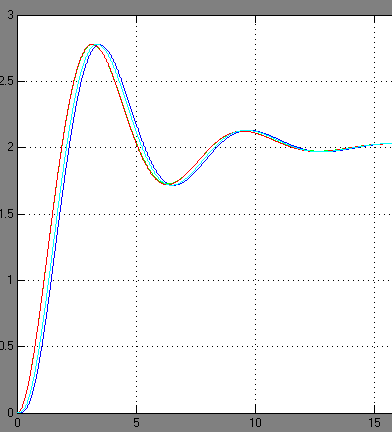
\includegraphics[scale=0.5]{figure17.png}
	\caption{Simulación, comparación modelos y respuesta real}
	\label{fig17}
\end{figure}

\subsection{Análisis de respuesta transitoria y modelado experimental del motor LEGO}
\noindent
A partir de la información obtenida del NXT se muestra en la Fig. \ref{fig1}, como es el comportamiento de la velocidad angular del motor respecto al tiempo:
\begin{figure}[H]
	\centering
		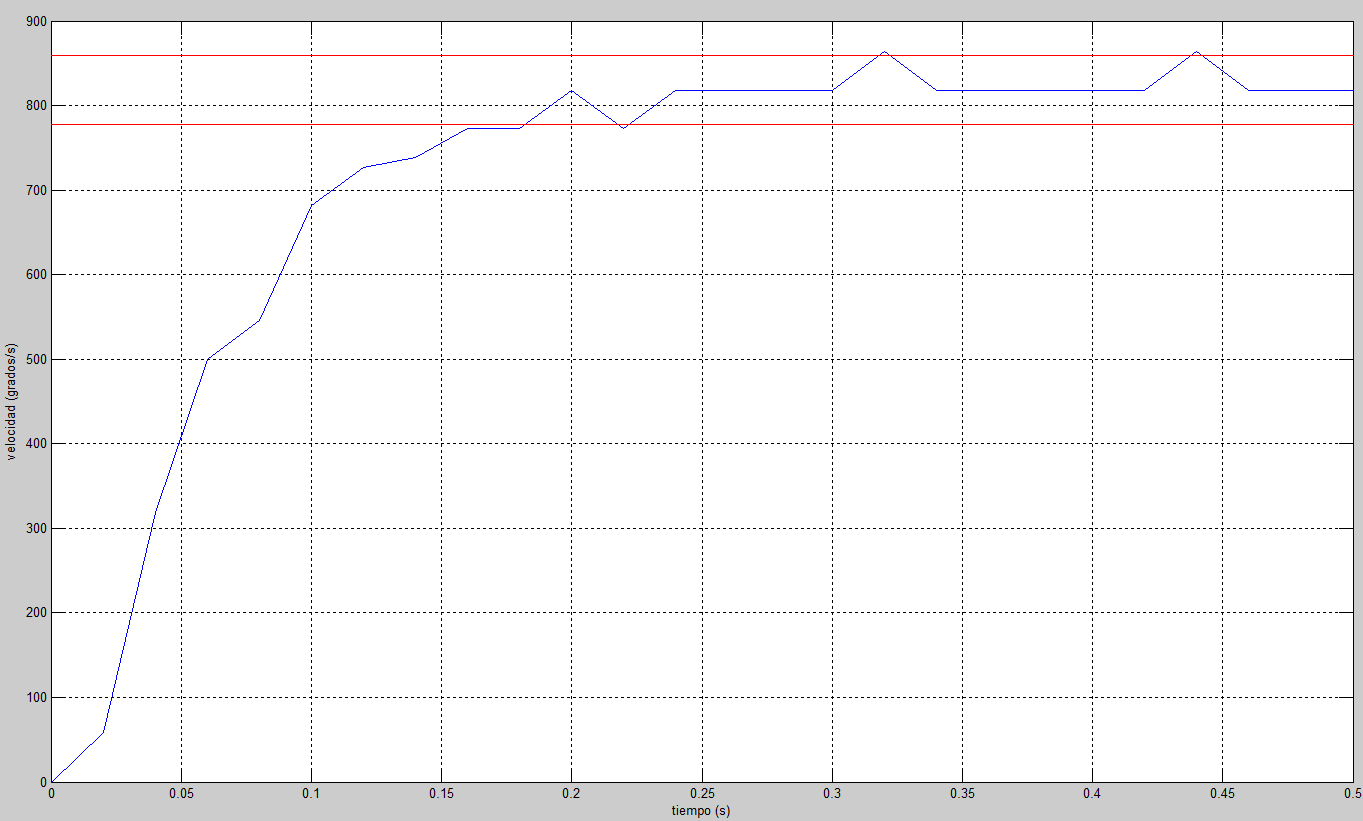
\includegraphics[scale=0.17]{figure1.png}
	\caption{Velocidad Angular \textbf{VS.} Tiempo.}
	\label{fig1}
\end{figure}
\noindent
Teniendo en cuenta que el sistema recibe una entrada tipo paso con amplitud del $100\%$, con base a la gráfica de velocidad contra tiempo, se nota que el sistema tiene un comportamiento muy similar al de un sistema de primer orden y se puede realizar una aproximación a este tipo de sistemas, por medio del cálculo de los siguientes parámetros:
\begin{equation}
 k=\frac{\Delta Salida_{ss}}{\Delta Entrada_{ss}}
\label{ecu1}
\end{equation}
$$t_s=3 \tau=0.182s$$
$$\tau=0.061$$
\noindent
Con una banda de tolerancia de $\pm 5$ para el cálculo del tiempo de asentamiento ($t_s$) ecu.(\ref{ecu2})
\begin{equation}
 G_{1}(s)=\frac{8.181818}{0.061s+1}
\label{ecu2}
\end{equation}
\begin{figure}[H]
	\centering
		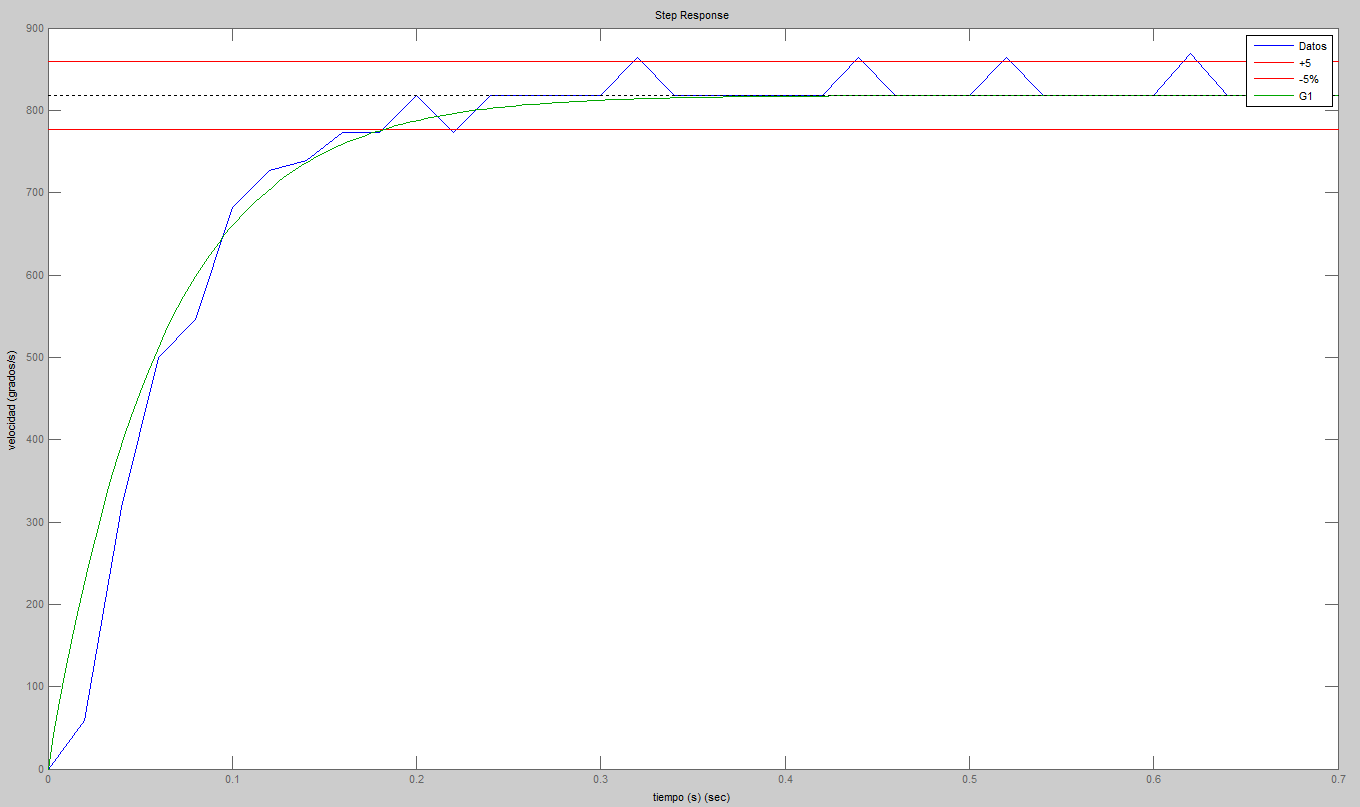
\includegraphics[scale=0.17]{figure2.png}
	\caption{Velocidad Angular \textbf{VS.} Tiempo.}
	\label{fig2}
\end{figure}

\subsubsection{Método de los  dos puntos}
\noindent
Este método permite identificar la respuesta de un sistema de primer orden a una entrada escalón, a partir de la respuesta real obtenida del sistema por medio de la identificación de dos puntos ubicados en la máxima región de cambio.
\begin{enumerate}
 \item Calcular el valor de la ganancia descrita por la ecu.(\ref{ecu1})
 \item Ubicar los puntos $t_1=(\theta+\frac{\tau}{3})$ y $t_2=\theta+\tau$; donde $\theta$ es el tiempo muerto a partir de las ecu.(\ref{ecu3}) y ecu.(\ref{ecu4})
\begin{equation}
 \Delta y(\theta+ \tau)=0.632\Delta y_{ss}
\label{ecu3}
\end{equation}
\begin{equation}
 \Delta y(\theta +\frac{\tau}{3})=0.283\Delta y_{ss}
\label{ecu4}
\end{equation}
\noindent
Donde a $$0.632\Delta y=517.09,\leq corresponde\ \ el \ \ tiempo\ \ t_2=0.0675$$\\
Donde a $$0.283\Delta y=231.54,\leq corresponde\ \ el \ \ tiempo\ \ t_2=0.0333$$
\begin{figure}[H]
	\centering
		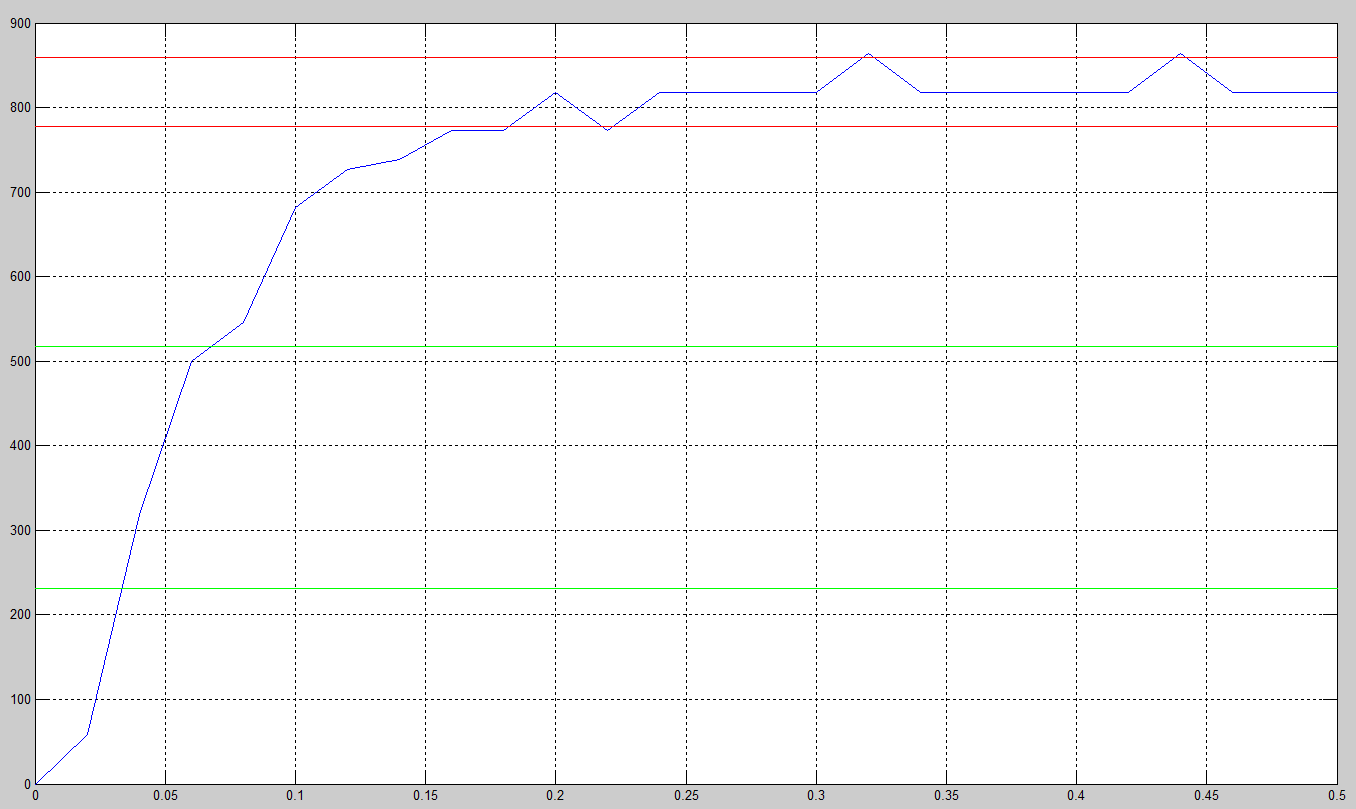
\includegraphics[scale=0.17]{figure3.png}
	\caption{Velocidad Angular \textbf{VS.} Tiempo.}
	\label{fig3}
\end{figure}
 \item A partir de los puntos anteriores se calcula:
\begin{equation}
 \tau=\frac{3}{2}(t_2-t_1)=\frac{3}{2}(0.0675-0.0333)=0.0513s
\label{ecu5}
\end{equation}
$$\theta =0.0675-0.0513=0.0162s$$
\end{enumerate}
\noindent
La función de transferencia correspondiente es ecu.(\ref{ecu6})
\begin{equation}
 G_2(s)=\frac{8.1818}{0.0513s+1}e^{-0.0162s}
\label{ecu6}
\end{equation}
\noindent
La siguiente figura muestra la respuesta de la función $G_2$ sin el tiempo muerto, y como es su comportamiento respecto a los datos y la función anterior
\begin{figure}[H]
	\centering
		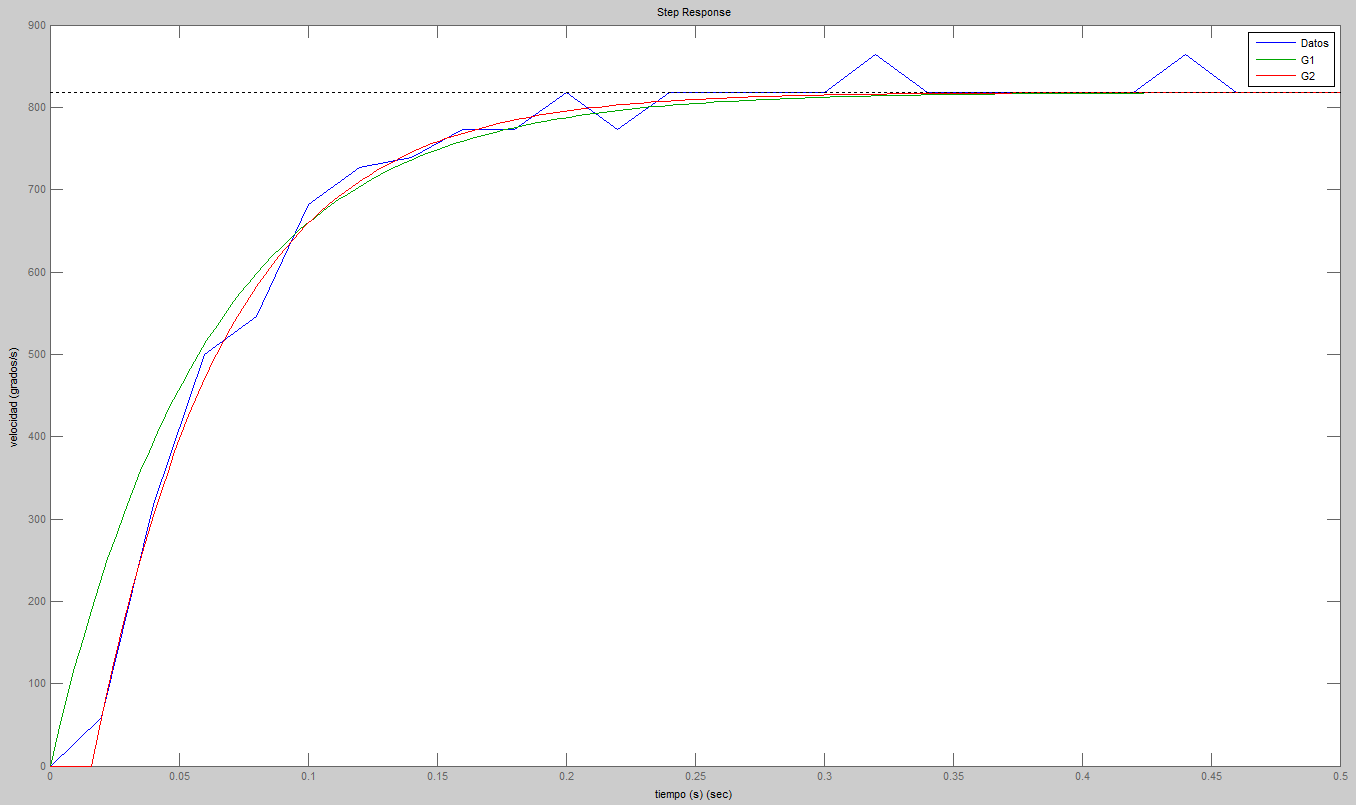
\includegraphics[scale=0.17]{figure4.png}
	\caption{Velocidad Angular \textbf{VS.} Tiempo.}
	\label{fig4}
\end{figure}

\subsubsection{IDENT}
\noindent
Los datos experimentales cargados en la herramienta Ident se muestran en la Fig. \ref{fig5}
\begin{figure}[H]
	\centering
		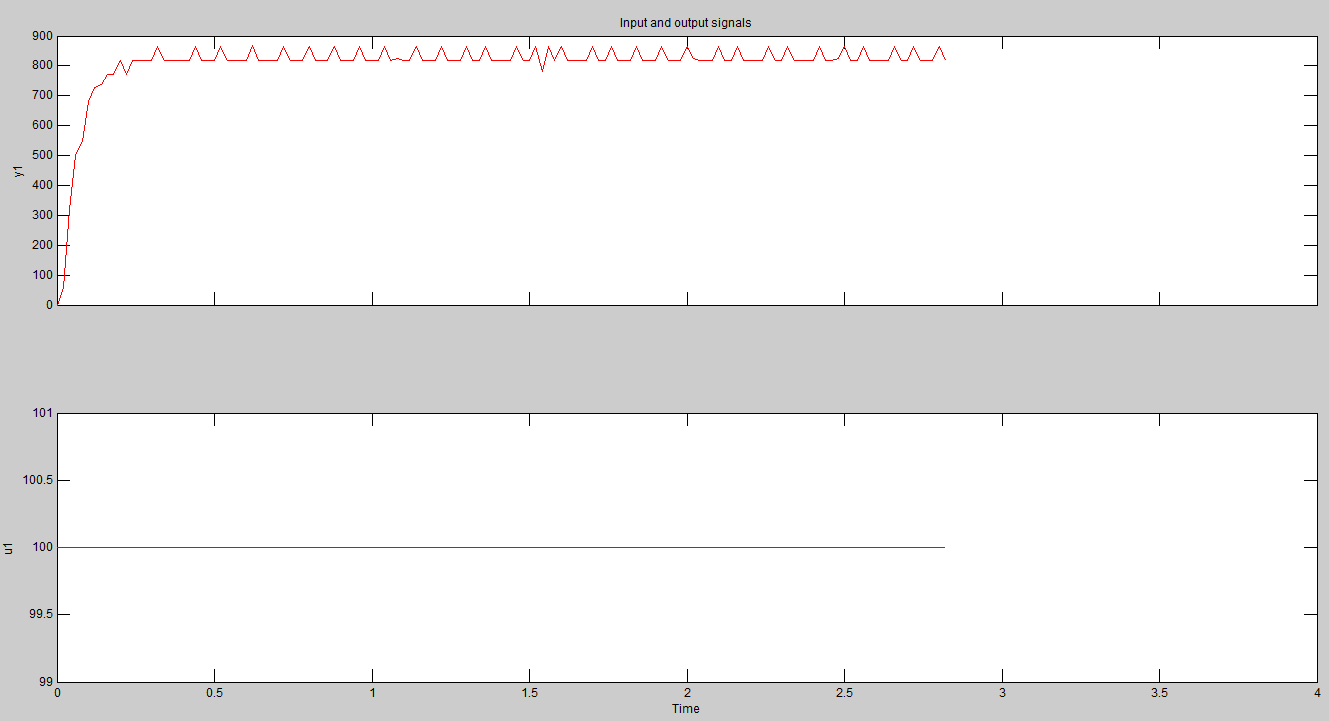
\includegraphics[scale=0.17]{figure5.png}
	\caption{Figura de la Herramienta IDENT}
	\label{fig5}
\end{figure}
\noindent
Por medio de la herramienta de identificación Ident se construyen la siguiente función de transferencia ecu.(\ref{ecu7})
\begin{equation}
 G_3(s)=\frac{8.3064}{1+0.069502s}=\frac{K_p}{1+T_p s}
\label{ecu7}
\end{equation}
\noindent
La función $G_3$ al ser comparada con los datos se muestra en la siguiente figura, donde la herramienta calcula un nivel de aproximación del $78.81\%$ Fig. \ref{fig6}
\begin{figure}[H]
	\centering
		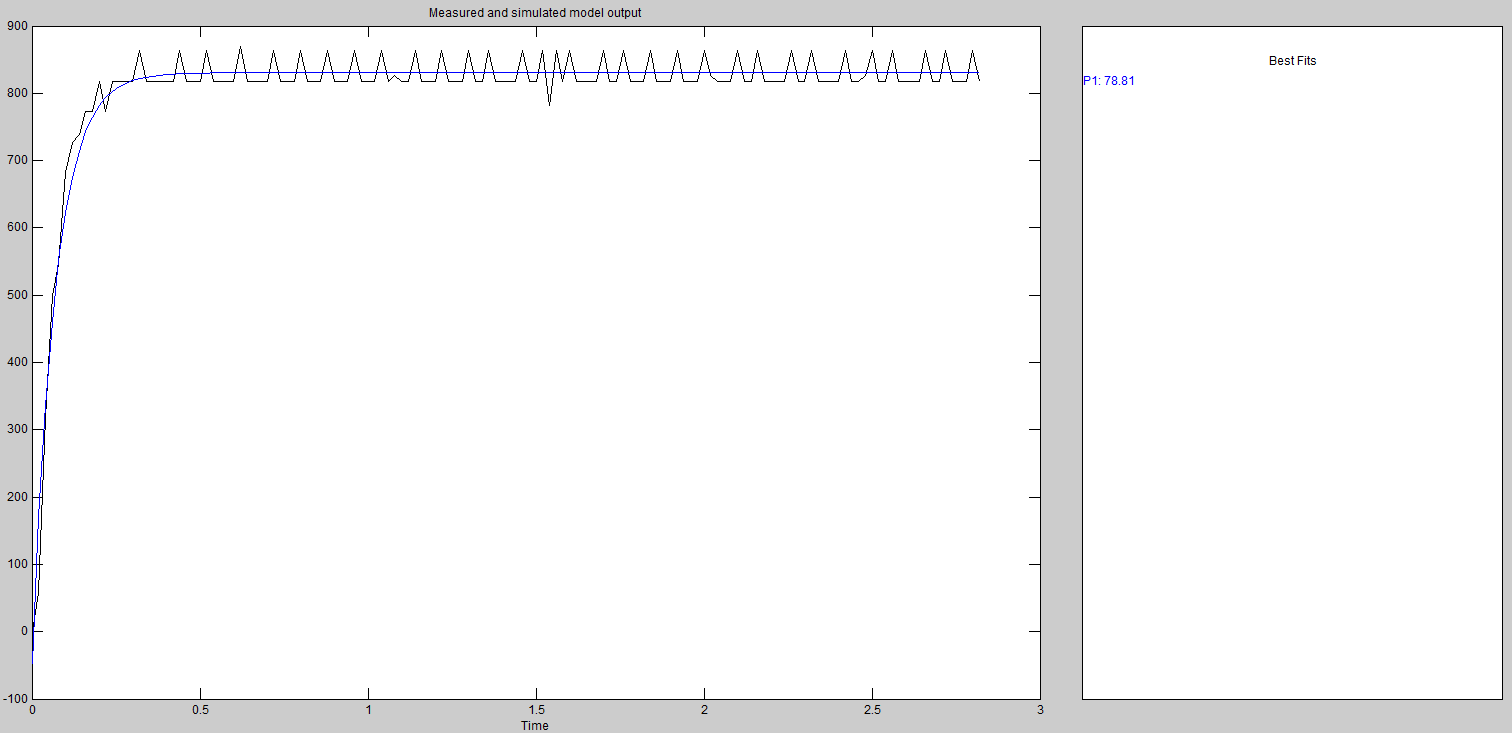
\includegraphics[scale=0.17]{figure6.png}
	\caption{Figura de la Herramienta IDENT}
	\label{fig6}
\end{figure}
\noindent
4. La simulación en Simulink por medio de diagrama de bloques muestra el siguiente resultado, comparando cada una de las funciones de transferencia con los datos experimentales
\begin{figure}[H]
	\centering
		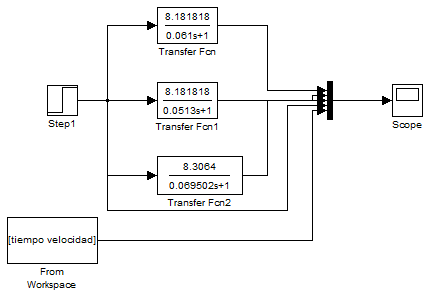
\includegraphics[scale=0.5]{figure7.png}
	\caption{Diagrama de bloques (Simulink)}
	\label{fig7}
\end{figure}
\begin{figure}[H]
	\centering
		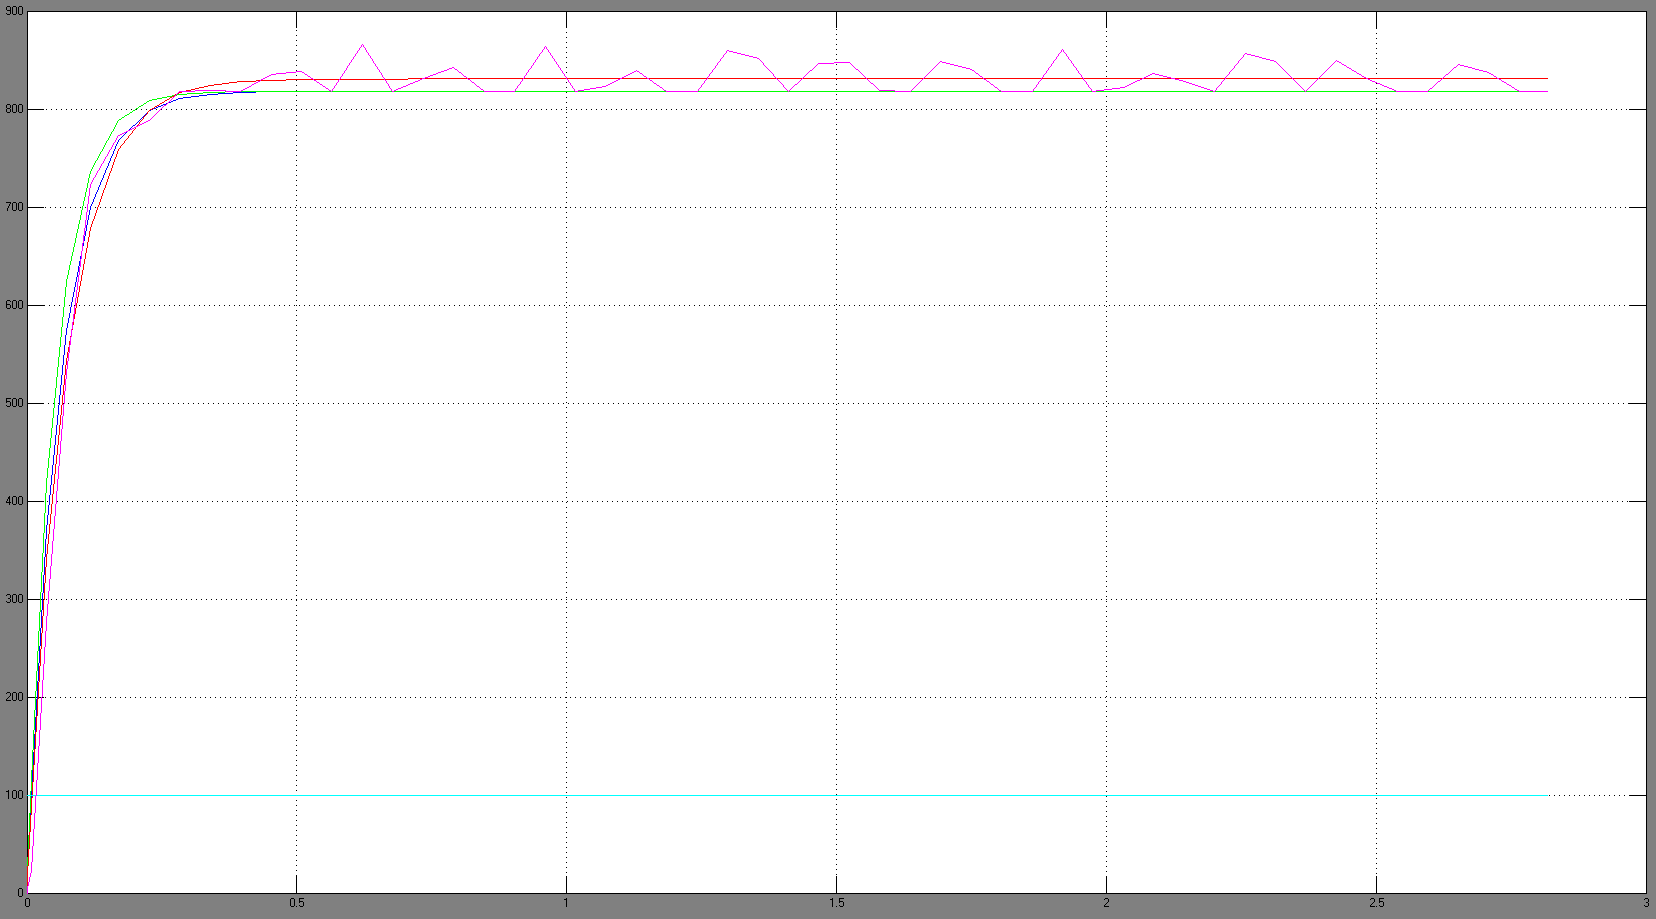
\includegraphics[scale=0.15]{figure8.png}
	\caption{Señales de Salida mostradas por el Scope}
	\label{fig8}
\end{figure}
\noindent
Se evalúan los tres modelos obtenidos por medio del índice del error cuadrático medio, el cual corresponde a la ecu.(\ref{ecu8})
\begin{equation}
E = \sqrt {\frac{{\sum\limits_{i = 1}^n {\left( {y_i  - d_i } \right)} ^2 }}{n}}
\label{ecu8}
\end{equation}
\noindent
Siendo $d_i$ los valores tomados experimentalmente, y $y_i$ el valor correspondiente de la salida obtenida a partir de la función de transferencia evaluada. Este índice permite obtener un criterio de evaluación para la magnitud del error estimado entre el modelo obtenido y los datos reales. A partir de los cálculos obtenidos se encuentra que el modelo de la función de transferencia $G_1$ tiene un índice de $165.2080$, el modelo obtenido a partir de $G_2$ tiene un índice de $232.5671$ y el modelo de $G_3$ muestra un índice de $165.2080$, por lo que el tercer modelo muestra una mejor aproximación al comportamiento experimental, aunque el primer modelo también permite una buena aproximación.

\subsection{Modelado de Motores DC}
\noindent
La simulación del sistema del motor LEGO por medio de diagrama de bloques, con los valores proporcionados por el enunciado, se muestra a continuación Fig. \ref{fig9}
\begin{figure}[H]
	\centering
		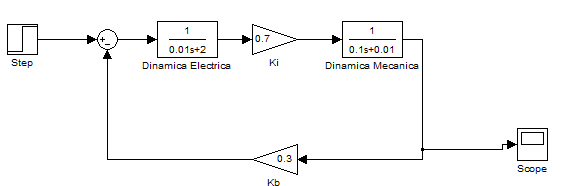
\includegraphics[scale=0.4]{figure9.png}
	\caption{Diagrama de Bloques del motor LEGO}
	\label{fig9}
\end{figure}
\noindent
La simulación muestra la siguiente respuesta a una entrada paso de amplitud $1V$ Fig. \ref{fig10}
\begin{figure}[H]
	\centering
		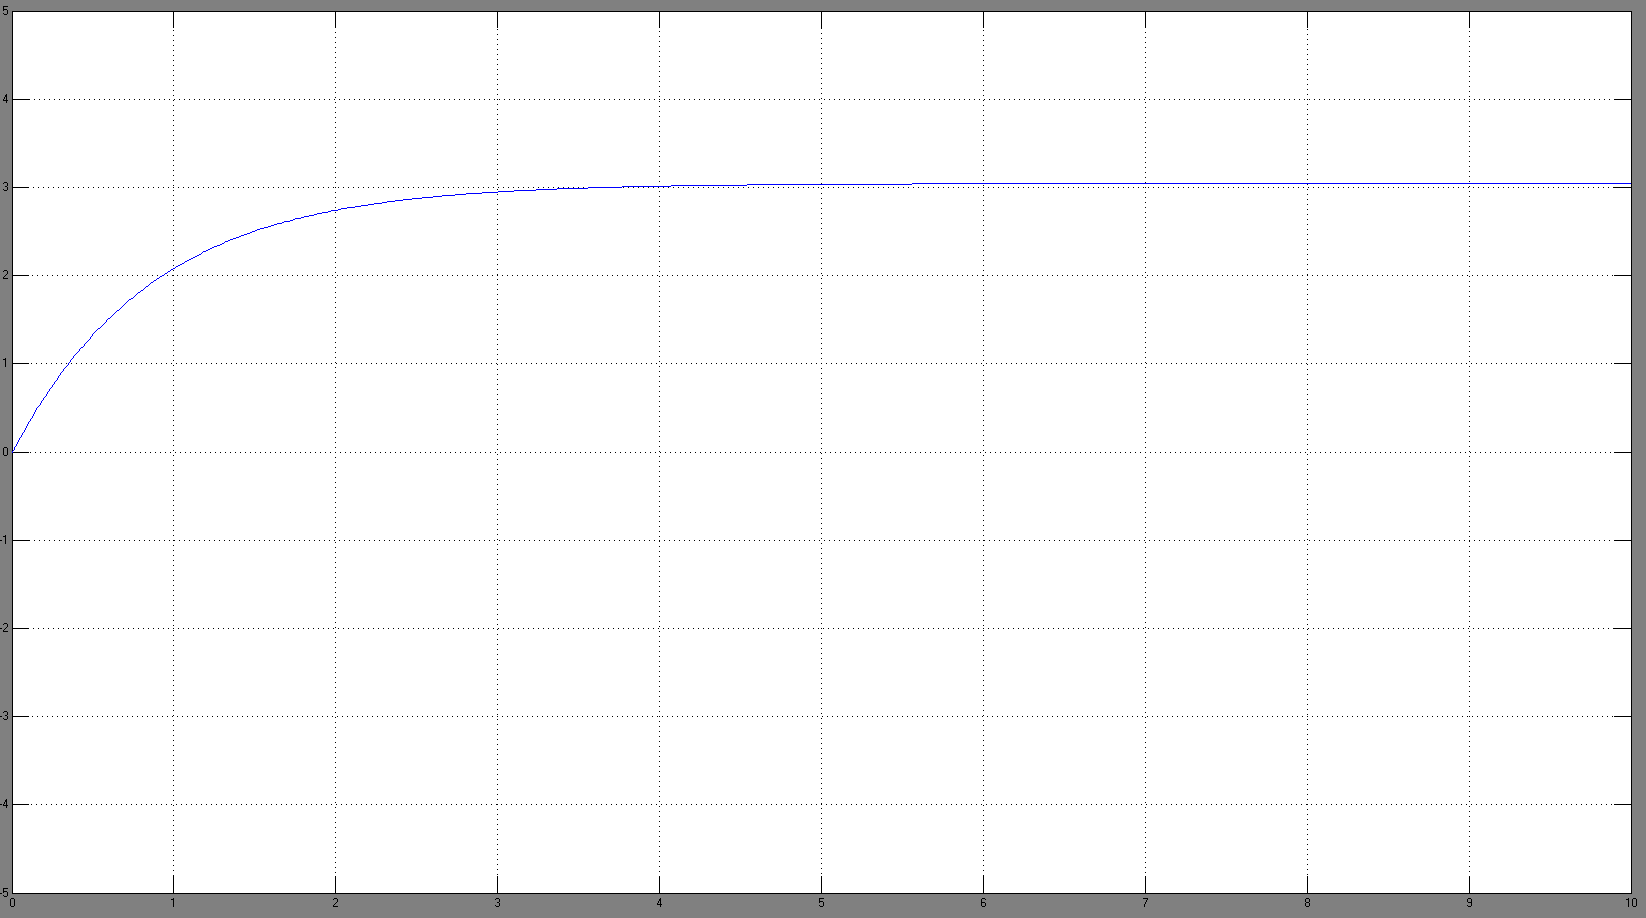
\includegraphics[scale=0.15]{figure10.png}
	\caption{Respuesta del sistema frente a una entrada paso}
	\label{fig10}
\end{figure}
\noindent|
Se observa que aunque el sistema está constituido por dos dinámicas diferentes proporcionados por la dinámica eléctrica representada en el circuito de la armadura del motor, y la dinámica mecánica que constituyen los torques que se desarrollan en el eje del motor, la respuesta del sistema es bastante similar a la respuesta de un sistema de primer orden ante una entrada paso.\\
Esto se debe a que los tiempos de respuesta de la etapa eléctrica del sistema son mucho mayores que la etapa mecánica, por lo que los polos proporcionados por esta última etapa son los dominantes y determinan la mayoría de la dinámica del sistema. La gran diferencia entre los tiempos de respuesta de las dos dinámicas, causan que el dominio de los polos sea bastante mayor, por lo que los polos no dominantes no causan mucho efecto en el sistema, y este sea asemeje a un sistema de primer orden.\\\\
La función de transferencia general del sistema  es la siguiente
\begin{equation}
 G_0(s)=\frac{0.7}{0.001s^2+0.2s+0.23}
\end{equation}
\noindent
Esta función de transferencia se puede visualizar como
\begin{equation}
 G_0(s)=\frac{0.7}{0.001(s+1.15669)(s+198.843)}
\end{equation}
\noindent
Como se puede observar los polos del sistema se encuentran en $1.15669$ y $198.843$, donde el polo dominante es el primero.\\\\
Hay dos formas de reducir el orden de un sistema: 
\begin{enumerate}
 \item Por aplicación de la teoría de polos dominantes. Los  polos ubicados en la región de insignificantes pueden ser eliminados.
 \item Mediante la cancelación entre el efecto de un polo y un  cero próximo entre sí.
\end{enumerate}
\noindent
En este caso se reduce la función de transferencia eliminando el polo menos dominante en $G(s)$, sin embargo la ganancia no tiene que verse afectada por lo cual:
\begin{equation}
 G_r(s)=\frac{K_p}{s+1.1561}
\end{equation}
\begin{equation}
 \mathop {\lim }\limits_{s \to 0} G(s) = \mathop {\lim }\limits_{s \to 0} G_{eq} (s)
\end{equation}
$$\frac{0.7}{0.23}=\frac{K_p}{1.1561}$$
\noindent
Ganancia $K_p=3.5186$. Finalmente se tiene que la función de transferencia reducida es:
\begin{equation}
 G_r(s)=\frac{3.5186}{s+1.1561}
\label{ecu9}
\end{equation}
\noindent
A continuación se muestra la respuesta escalón de ambos modelos, en azul el sistema original $G(s)$ y en verde el sistema reducido $G_r(s)$. 
\begin{figure}[H]
	\centering
		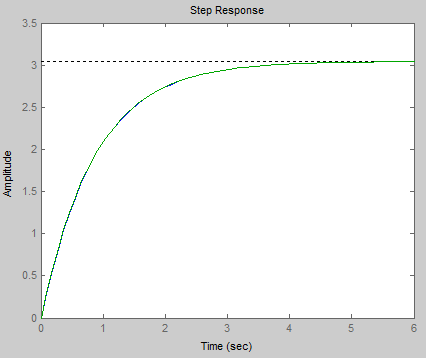
\includegraphics[scale=0.5]{figure11.png}
	\caption{Respuesta escalón, sistema original y reducido}
	\label{fig11}
\end{figure}
\begin{figure}[H]
	\centering
		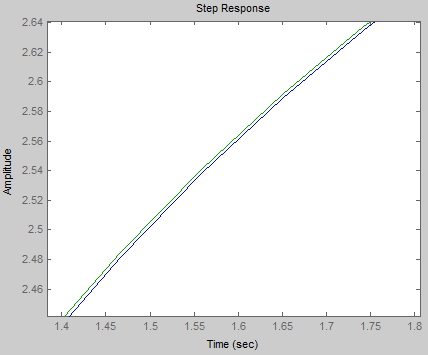
\includegraphics[scale=0.5]{figure12.png}
	\caption{Análisis detallado modelo original y reducido}
	\label{fig12}
\end{figure}
\noindent
De las figuras Fig. \ref{fig11} y Fig. \ref{fig12} se observa que la reducción hecha en $G(s)$ es bastante buena, esto gracias a que el polo eliminado se encuentra muy alejado del eje imaginario por lo que tiene muy poca influencia en la respuesta transitoria del sistema, y la respuesta estacionaria es controlada mediante el ajuste en la ganancia. Finalmente se concluye que el modelo reducido es el mejor para modelar este sistema, gracias su sencillez y su gran semejanza con el original.

\section{Conclusiones}
\begin{itemize}
 \item La caracterización de un sistema a partir de datos experimentales, permiten aproximar matemáticamente la dinámica del sistema y construir un modelo representativo del sistema, que permite predecir el comportamiento frente a diferentes tipos de entradas o perturbaciones.
 \item La determinación de un modelo (función de trasferencia en este caso) es muy importante a la hora de describir un sistema, pues gracias a este se puede predecir su comportamiento además de analizar sus límites, su respuesta ante diferentes entradas y sus puntos de estabilización.
 \item En general, un sistema puede ser modelado mediante funciones de trasferencia de diferentes ordenes, por lo general entre mayor orden mejor se describe el sistema, aunque en la mayoría de casos es más practico reducir dichas funciones para obtener modelos matemáticos más simples y sencillos de analizar, eso sí, siempre y cuando la reducción sea justificada y se acerque en buena medida a el modelo original.
\end{itemize}

\bibliographystyle{ieeetran}
\begin{thebibliography}{99}

\bibitem{chen} Chen, Chi-Tsong.
{\em "`Analog and Digital Control System Desing: Transfer-Function, State, Space and Algebraic Methods"'}.
Saunders College Publishing, 1993.

\bibitem{page1} Sitio Web: \url{http://www.disa.bi.ehu.es/spanish/asignaturas/17211/Practica2.pdf}

\bibitem{page1} Sitio Web: \url{http://www.elai.upm.es:8009/spain/Asignaturas/Servos/Apuntes/7_OrdenSup.pdf}

\end{thebibliography}
\end{document}